\section{Systems with inputs and outputs}

Study/control systems $\dot{x} = f(x,u)$ with "output" $y(t)=h(x(t))$

\subsection{Sliding mode control}

Motivating example
\begin{equation*}
\left\{
                \begin{array}{l}
                  \dot{x_1} = x_2\\
                  \dot{x_2} = u \\
                  y = x_1 + x_2
                \end{array}
              \right. 
\end{equation*}
$\Rightarrow \dot{y} = x_2 + u$

Choose:
\begin{equation*}
u =  \left\{
                \begin{array}{ll}
                  -x_2-1, \ \ y > 0\\
                  -x_2+1, \ \ y < 0\\
                  -x_2, \ \ y=0
                \end{array}
              \right. 
\end{equation*}
\begin{equation*}
\Rightarrow \dot y =  \left\{
                \begin{array}{ll}
                  -1, \ \ y > 0\\
                  +1, \ \ y < 0\\
                  0, \ \ y=0
                \end{array}
              \right. 
\end{equation*}

Solutions(Laratheodory) are if $y(0) > 0$, then 
\begin{equation*}
y(t) = \left\{ \begin{array}{ll}
                  y(0) - t, \ \ t \leq y(0)\\
                  0, \ \ t > y(0)
                \end{array}
              \right. 
\end{equation*}
If $y(0) < 0$, then
\begin{equation*}
y(t) = \left\{ \begin{array}{ll}
                  y(0) + t, \ \ t \leq y(0)\\
                  0, \ \ t > -y(0)
                \end{array}
              \right. 
\end{equation*}

\begin{center}
	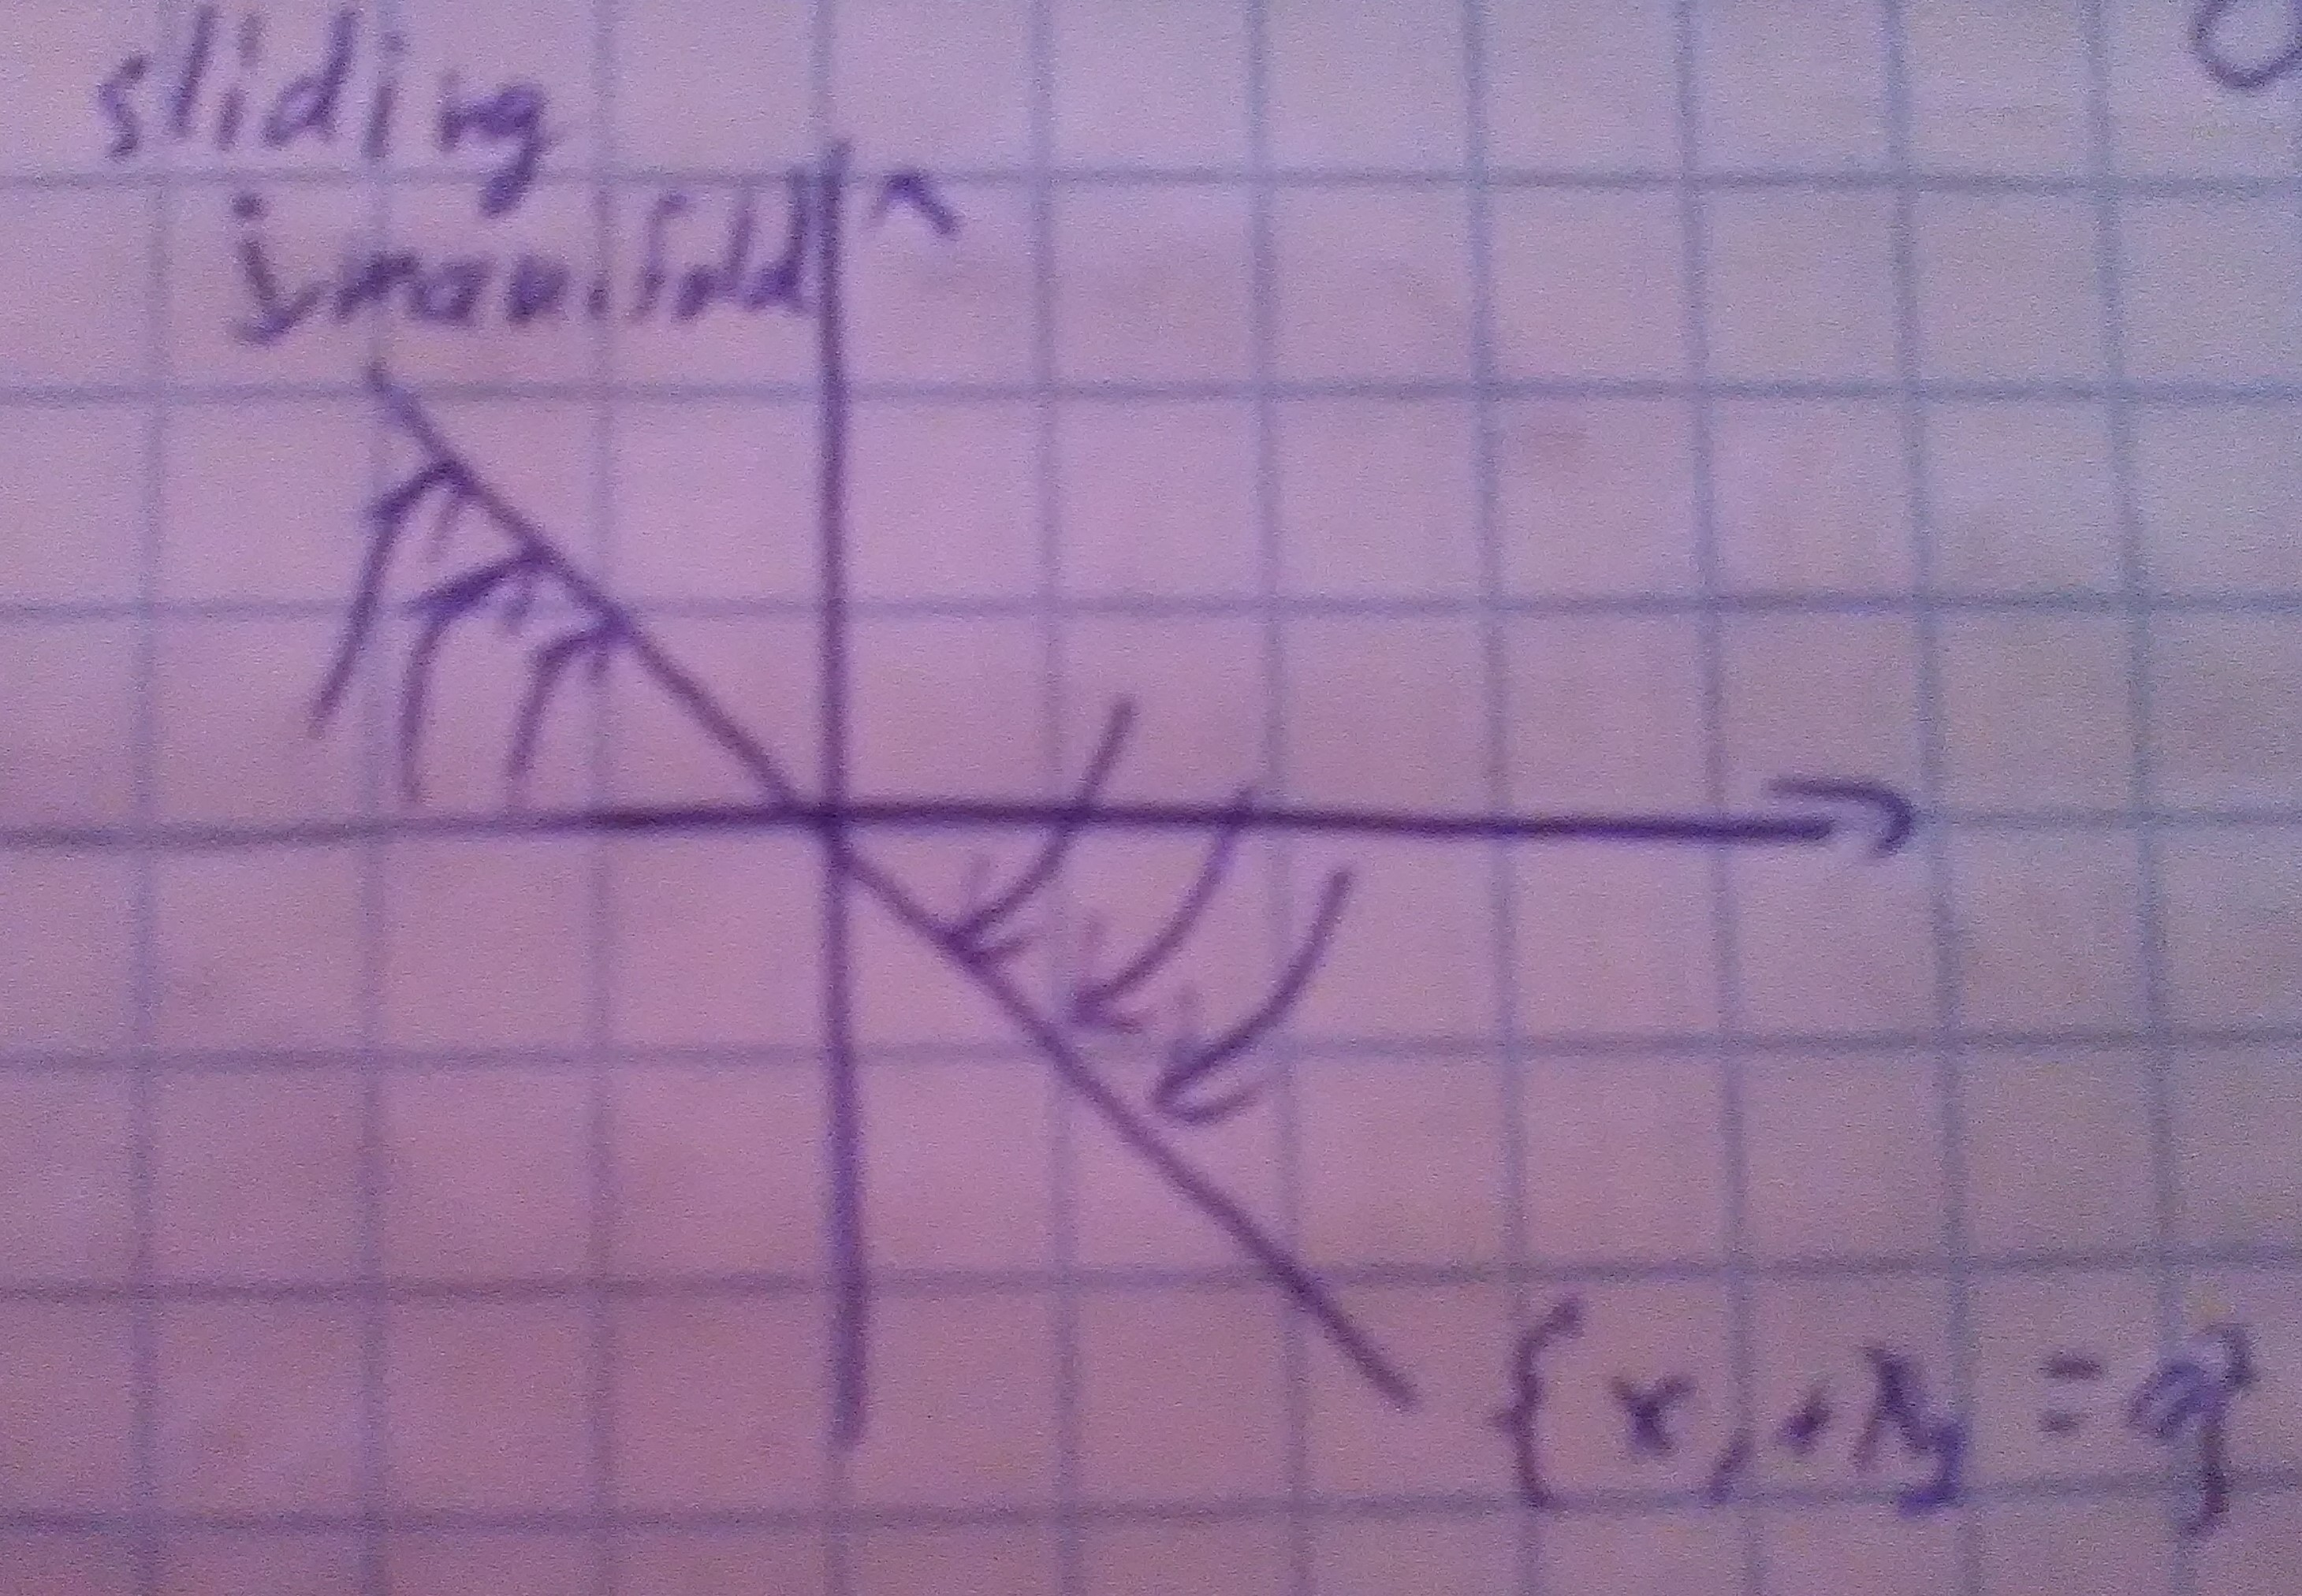
\includegraphics[scale=0.1]{1}
\end{center}

Key property: choose $u$ s.t. $y(t)$ goes to zero in finite time $\Rightarrow x(t)$ tends $S := \{ (x_1, x_2) \in \mathbb{R}^2 | x_1 +x_2 = 0 \}$ in finite time

Consider dynamics on $S$
\begin{equation*}
\left\{ \begin{array}{l}
                  \dot{x_1} = x_2 (x_2 = -x_1 \ $if$ \  y =1) = -x_1\\
                 \dot{x_2} = u = -x_2
                \end{array}
              \right. 
\end{equation*} 
globally as stable

Two "phases"
\begin{enumerate}
\item solutions converge to $S$ in finite time
\item solutions converge to zero ("on S") asymptotically
\end{enumerate}
$\leadsto $ "sliding mode" control

Remark: in (1) "finite time convergence is crucial"

General procedure:
\begin{equation*}
\begin{split}
\dot{x} = f(x)+g(x)u \\
y = h(x)= s(x)
\end{split}
\end{equation*}
$f: \mathbb{R}^n \to \mathbb{R}^n, \  y : \mathbb{R}^n \to \mathbb{R}^n, \ s: \mathbb{R}^n \to \mathbb{R}$

$u$ - scalar input, $s(x)$ - sliding

single input, single output 

Assumptions: $y$ has relative degree 1, well - defined globally, i.e. $L_gs(x) \neq 0 \ \forall \in \mathbb{R}^n$

Two-step approach:
\begin{enumerate}
\item Bring $x(t)$ to $S := \left \{ x \in \mathbb{R}^n | S(x) = 0 \right\}$ in finite time
\item Have $x(t)$ going to zero asymptotically (on $S$)
\begin{itemize}
\item switching between nodes 1 and 2
\item mode 2 is "sliding mode"
\end{itemize}
\end{enumerate} 

\begin{center}
	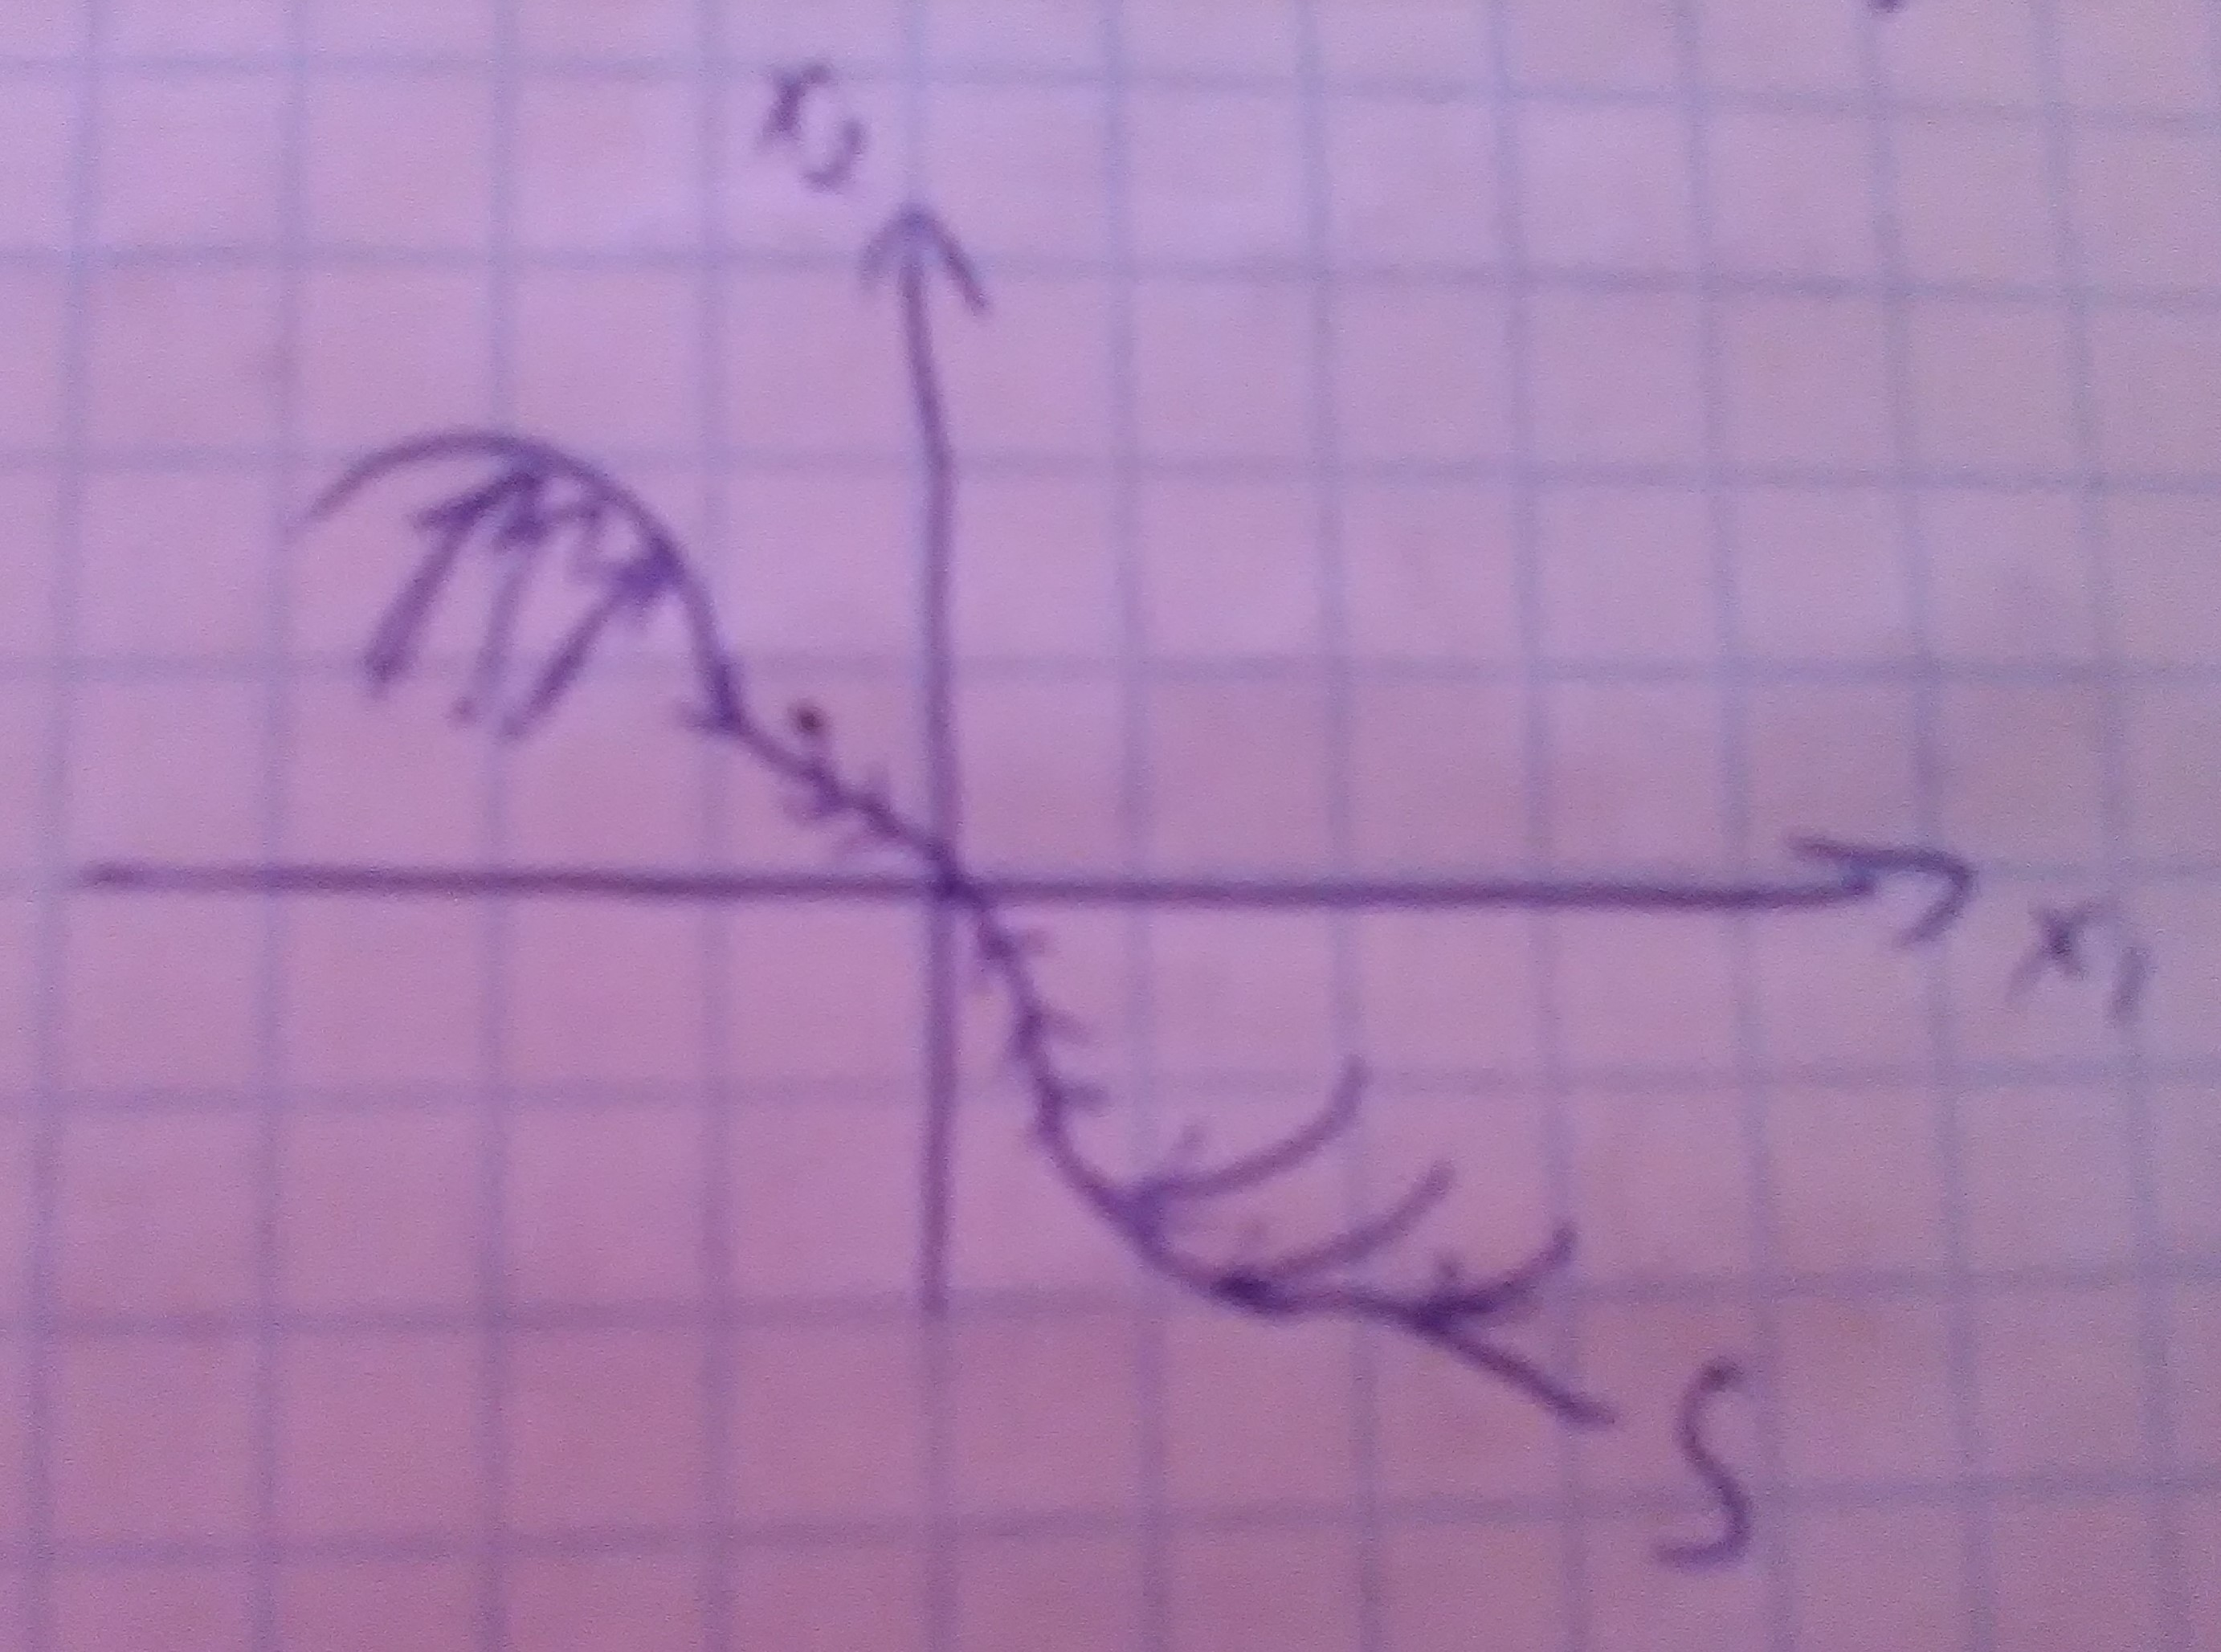
\includegraphics[scale=0.1]{2}
\end{center}

How are 1 + 2 achieved?
\begin{itemize}
\item Design of sliding manifolds crucial!

Need: For $y(t)=0$ for all $t \geq 0$. All solutions converge to the origin, i.e., "zero dynamics" have globally asymptotically stable origin.

How? e.g. systems in "regular form"
$x = \left[ \eta, \ \xi \right]'$ 
\begin{equation*}
\begin{array}{l}
     \dot{\eta} = f_1(\eta, \xi)\\
     \dot{\xi} = f_2(\eta, \xi) + g_2(\eta,\xi) u
\end{array}
\end{equation*}
Choose $s(x)=\eta - \phi(\eta)$, where $\phi$ asymptotically stabilizes zero dynamics $\dot{\eta} = f_1(\eta, \phi(\eta))$ (and $\phi(0) = 0$)
Ex. 1.9 in Khalil
\item Converging to sliding manifold in finite time:
$\leadsto \dot{s} = L_fs(x) + L_gs(x)u$, where $L_gs(x) \neq 0$. Obvious choice to render $S$ invariant is $u = - \frac{L_fS(x)}{L_gs(x)}$ (mode 2, behaviour on $S$)

Motivating example, add 
\begin{equation*}
\left \{ \begin{array}{ll}
     - \hat{u}/ L_gs(x) & y > 0 \\
     \hat{u} /L_gs(x) & y < 0
\end{array} \right.
\end{equation*}
where $\hat{u} > 0$

\begin{equation*}
 u = - \frac{1}{L_gs(x)}(L_fs(x) + \hat{u}sgn(s(x)))
\end{equation*}
$\leadsto \dot{y} = - \hat{u} sgn(y)$

$\leadsto $ (caratheodory) solutions converge to zero in finite time

$\leadsto x(t)$ converges to $S$ in finite time
\end{itemize}

Control Lyapunov perspective

$V(X) = \frac{1}{2}s(x)^2$
\begin{equation*}
\dot{V}(x) = s(x) \dot{s}(x) = s(x)(L_fs(x)+L_gs(x)u) = -s(x)sgn(s(x))\hat{u} = | s(x)|\hat{u} < 0,\ s(x) \neq 0
\end{equation*}

Consider $w = \sqrt{2v} \leadsto^{s \neq 0} \dot{w} = \sqrt{2}\frac{1}{2\sqrt{v}}\dot{v}=-\hat{u}$

$\leadsto w$ converges to 0 in finite time $\Rightarrow v $ converges to 0 in finite time $\Rightarrow S(x(t))$ converges to 0 in finite time.

\begin{Example}
\begin{equation*}
\begin{array}{l}
     \dot{x_1} = x_2 + x_1 sin(x_2)\\
     \dot{x_2} = x_2^2 + x_1 + u
\end{array}
\end{equation*}
Choose $s(x) = x_2 + 2x_1$, where $-2x_1 := \phi(x_1)$ on $S$: $\dot{x_1} = -2x_1 + x_1 sin(-2x_1) \leadsto $ asymptotically stable
\begin{equation*}
\dot{s} = x_2^2 + x_1 + u + 2x_2 + 2x_1 sin(x_2) \leadsto u = - (x_2^2 + x_1 +2x_2+2x_1sin(x_2) + \hat{u}sgn(x_2 + 2x_1)), \ \hat{u} > 0
\end{equation*} 
$\leadsto$ yields finite-time convergence to $S$.
\end{Example}

Alternative sliding mode controllers
\begin{equation*}
u = - \frac{1}{L_gs(x)}(L_fs(x) + \hat{u}sgn(s(x))), \ \hat{u} > 0
\end{equation*}

In particular
\begin{equation*}
u = - \frac{1}{L_gs(x)}(L_fs(x) + \hat{u}|L_gs(x)|sgn(s(x)))
\end{equation*}
$\leadsto $ ensure robustness w.r.t. "matched uncertainties"
\begin{equation*}
\dot{x} = f(x) + g(x) \sigma (x) + g(x)u 
\end{equation*}
$\sigma : \mathbb{R}^n \to \mathbb{R}$, bounded (i.e., $|\sigma (x)| \leq c \ \forall x \in \mathbb{R}^n $)

Why? $V(x) = \frac{1}{2}s(x)^2$
\begin{equation*}
\dot{V} = s(x)(L_fs(x) + L_gs(x)u + L_gs(x)\sigma (x)) = - s(x)sgn(s(x)) \hat{u} |L_gs(x)| + s(x)L_gs(x)\sigma (x) \leq - |s(x)| |L_gs(x)| (\hat{u} - c)
\end{equation*}
\begin{equation*}
u = - \frac{1}{L_gs(x)}(L_fs(x) + (\hat{u} + \beta (x) |L_gs(x)|) sgn(s(x)))
\end{equation*}
ensures robustness w.r.t. matched uncertainties s.t. $\sigma (x) \leq \beta (x) \ \forall x\in \mathbb{R}^n$

\begin{Example}
\begin{equation*}
\begin{array}{l}
     \dot{x_1} = x_2 + x_1 sin(x_2)\\
     \dot{x_2} = \theta x_2^2 + x_1 + u
\end{array}
\end{equation*}

$|\theta| \leq 2 \leadsto |\theta x_2^2| \leq 2x_2^2 = \beta(x)$

\begin{equation*}
\dot{s} = \theta x_2^2 + x_1 +u +2x_1 +2x_1sinx_2
\end{equation*}
\begin{equation*}
u = -(x_1 +2x_1 +2x_1sinx_2 + \hat{u}sign(s(x)) + 2x_2^2sgn(s(x)))
\end{equation*}
$L_fs(x) = x_1 +2x_1 +2x_1sinx_2$

$\leadsto \dot{s} = - \hat{u}sgn(s(x)) + x_2^2(\theta - 2sgn(s(x))) \Rightarrow$ finite -time convergence to $S$.
\end{Example}

Remedy: replace sign-function by saturated slope (continuous approximation)

can be extended to multi-input systems $u \in \mathbb{R}^m \to s: \mathbb{R}^n \to \mathbb{R}^m$

\subsection{Dissipativity}

Dissipativity: Generalization of Lyapunov theory to systems $w$ inputs and outputs

\begin{equation}\label{input-output}
\begin{array}{lll}
     \dot{x} = f(x,u) & x(0) = x_0 & f: \mathbb{R}^n \times \mathbb{R}^m \to \mathbb{R}^n \\
     y = h(x) & & h: \mathbb{R}^n \to \mathbb{R}^p
\end{array}
\end{equation}

Definition: 
\begin{itemize}
\item storage function $S: \mathbb{R}^n \to \mathbb{R}$, $x \to S(x)$ nonnegative (i.e., $S(x) \geq 0 \ \forall x \in \mathbb{R}^n$)
\item supply rate $s: \mathbb{R}^m \times \mathbb{R}^p \to \mathbb{R}$, $(u,y) \to s(u,y)$
\end{itemize}

Definition: System (\ref{input-output}) is dissipative w.r.t. the supply rate $s$ if there exists a storage function $S$ s.t. $\forall x_0 \in \mathbb{R}$, $\forall t \geq 0$, $\forall u : [0, t] \to \mathbb{R}^m$

\begin{equation}\label{DIE}
S(x(t)) \leq S(x_0)
 + \int_0^ts(u(\tau), y(\tau))d\tau
\end{equation}  

First item - storage at time $t$, second item - initial storage,the last item - supply delivered over [0, $t$]

"dissipation inequality" (DIE) is the inequality (\ref{DIE})

Interpretation:
\begin{itemize}
\item "Dissipative systems dissipate storage/stored energy"
\item "No storage/energy can be created internally"
\item positive $s$ "supplied" energy/ storage
     
      negative $s$ "extracted" energy / storage
\end{itemize}

Remark: 
\begin{itemize}
\item If $S$ is differentiable, DIE is equivalent to $\dot{S}(x) \leq s(u,y) \ \forall u, x$
\item Dissipation (rate) is defined as $d(x,u) = s(u,h(x)) - \dot{S}(x) \geq 0$
\end{itemize}

Examples of dissipative systems:
\begin{center}
    \begin{tabular}{| l | l | l | l | l |}
    \hline
     & supply rate & input & output & storage function  \\ \hline
    electrical & $u \cdot i$ & voltage & current & energy storage in all capacitors and inductors\\ \hline
    mechanical & $F \cdot V$ & force & velocity & Hamiltonian = kinetic + potential energy \\ \hline
    thermo-dynamics & $Q + W$ & rate of hate & rate of work & internal energy \\
    \hline
    & $-\frac{a}{T}$ & & temperature & entropy \\
    \hline
    \end{tabular}
\end{center}

How do we computer storage functions?
\begin{itemize}
\item in general difficult (similar to computing Lyapunov functions)
\item characterization via optimization problem
\end{itemize}

Introduce "available storage"
\begin{equation*}
S_a(x) := sup_{u:[0,T] \to \mathbb{R}^m, T \geq 0, x(0) = 0} (- \int_0^Ts(u(\tau),y(\tau)))
\end{equation*}

the maximum of energy we can extract

\begin{Theorem}
System (\ref{input-output}) is dissipative w.r.t. the supply rate $s$ iff $S_a(x) < \infty$ for all $x \in \mathbb{R}^n$

Moreover, if $S_a(x) < \infty$ for all $x \in \mathbb{R}^n$, then $S_a$ is a storage function and $S(x) \geq S_a(x) \ \forall x \in \mathbb{R}^n$ for all storage functions $S$.

\begin{proof}
Sketch of proof. "$S_a(x) < \infty \Rightarrow$ dissipativity". $S_a(x) \geq 0 \ \forall x \in \mathbb{R}^n$ by definition (can take $T=0$)
\begin{equation*}
\begin{split}
S_a(x) = sup_{u[0,T] \to \mathbb{R}^m, T \geq 0, x(0) = 0}- \int_0^Ts(u(\tau), y(\tau))d\tau \geq^* \\ 
- \int_0^t s(u(\tau), y(\tau))d\tau + sup_{u[t,t+T] \to \mathbb{R}^m, T \geq 0, x(t) = x(t)} - \int_t^{t+T}s(u(\tau), y(\tau))d\tau
\end{split}
\end{equation*} 
the last item is $S_a(x(t))$, 
\begin{equation*}
\Rightarrow = S_a(x(t)) - \int_0^ts(u(\tau), y(\tau))d\tau
\end{equation*}
and this is DIE $\Rightarrow S_a$ is a storage function

Note for (*): "suboptimal" to first transfer system to $x(t)$ and then extract maximum energy starting of $x(t)$

"Dissip. $\Rightarrow S_a(x) < \infty$"

From DIE: $S(x_0) \geq S(x(T)) - \int_0^Ts(u(\tau), y(\tau))d\tau \geq - \int_0^T s(u(\tau),y(\tau))d\tau$

for all $x_0$, for all $T \geq 0$, all $u(\cdot) \Rightarrow S(x_0) \geq sup_{u:[0,T] \to \mathbb{R}^m, \ T \geq 0, \ x(0) = x_0} - \int_0^Ts(u(\tau),y(\tau))d\tau = S_a(x)$

$\Rightarrow S_a(x) < \infty \ \forall x \in \mathbb{R}^n$ and $S \geq S_a$ for all storage function $S$. 
\end{proof}
\end{Theorem}

Another special supply rate: "required supply"

\begin{equation*}
S_r(x) := inf_{u:[-T,0] \to \mathbb{R}^m, \ T \geq 0, \ x(-T) = x^*, \ x(0) = x} \int_{-T}^0 s(u(\tau), y(\tau))d\tau
\end{equation*}

\begin{Theorem}
Assume that end state $x \in \mathbb{R}^n$ is readable from $x^*$. If system (\ref{input-output}) is dissipative w.r.t. the supply rate $s$, then for all storage functions $S$
\begin{equation*}
S(x) \leq S_r(x) + S(x^*) \ \forall \in \mathbb{R}^n
\end{equation*}
Furthermore, $S_r(x) + S(x^*)$ is a storage function.
\begin{proof}
Sketch of proof.

Consider $u:[-T,0] \to \mathbb{R}^n$ which transfers the system from $x^*$ to $x$
\begin{equation*}
S(x) - S(x^*) \leq[by\ DIE] inf_{u[-T,0] \to \mathbb{R}^n, \ T \geq 0, \ x(-T) = x^*, \ x(0) = x} \int_{-T}^0 s(u(\tau), y(\tau))d\tau = S_r(x)
\end{equation*}
\end{proof}
\end{Theorem}

Remark: Set of all storage functions is convex, i.e. , $\alpha S_1 + (1-\alpha) S_2$, $\alpha\in [0,1]$ is a storage function (for $S1, \ S2$ storage functions)

Dissipativity widely used in control theory

If system is dissipative with positive definite storage $S$ and if there exists a (continuous) $k: \mathbb{R}^n \to \mathbb{R}^n$ s.t. 
\begin{equation*}
s(k(x),h(x)) < 0, \ \forall x \neq 0
\end{equation*}
then $x=0$ is asymptotically stable under $u=k(x)$

Why? Take $S$ as Lyapunov function 
\begin{equation*}
\dot{S} \leq s(u,y) =^{u=k(x)} s(k(x),h(x)) < 0, \ \forall x \neq 0
\end{equation*}

$L_2$ - gain via supply rate 
\begin{equation*}
s(u,y) = \frac{1}{2} \gamma^2 \|u\|^2 - \frac{1}{2}\|y\|^2
\end{equation*}
$\leadsto $ from dissipation inequality

\begin{equation*}
\begin{split}
\frac{1}{2} \int_0^t \gamma^2 \|u(\tau)\|^2 - \|y(\tau)\|^2d\tau \geq S(x(t)) - S(x(0)) \geq -S(x(0)) \\
\Rightarrow \int_0^t \|y(\tau)\|^2d\tau \leq \gamma^2 \int_0^t \|u(\tau)\|^2d\tau + 2 S(x(0)) \\
\end{split}
\end{equation*}
$\Rightarrow$ system has $L_2$ - gain $\gamma$

Classify optional $l(x,u^{\leftarrow x})$ operating conditions $s(u,y) = l(x,u) - l(x^*,u^*)$ 

\begin{Example}
\begin{equation*}
\dot{x} = u, \ y = x 
\end{equation*}
$S(x) = \frac{1}{2}x^2, \ \dot{S} = xu = uy \leadsto $ system is dissipative w.r.t. supply rate $s(u,y) = uy$.
\end{Example}

\begin{Example}
"part-Hamiltonian systems" 
\begin{equation*}
\dot{x} = [F(x) - R(x)] \triangledown H(x) + g(x)u
\end{equation*}
$y = g(x)^T\triangledown H(x)$, $H$ - Hamiltonian total stored energy in system

$F(x) = -F^T(x)$ internal interconnection structure (power conserving) $R(x) \geq 0$ dissipation structure

Take $S(x) = H(x)$
\begin{equation*}
\begin{split}
\dot{S}(x) = \triangledown H(x) \cdot [F(x) -R(x)]\triangledown H(x) + \triangledown H(x) \cdot g(x)u \\
= - \triangledown H(x) \cdot R(x) \triangledown H(x) + yu \leq yu 
\end{split}
\end{equation*}
as far as $- \triangledown H(x) \cdot R(x) \triangledown H(x) \leq 0 \Rightarrow$ dissipative w.r.t. $s(u,y) = u^Ty$   
\end{Example}

\subsection{Passivity}

\begin{equation}\label{passivity_system}
\begin{split}
\dot{x} = f(x,u), \ x \in \mathbb{R}^n, \ u \in \mathbb{R}^m \\
y = h(x), \ y \in \mathbb{R}^m
\end{split}
\end{equation}
(same number of inputs and outputs)

\begin{Definition}
System (\ref{passivity_system}) is passive if it is dissipative w.r.t. supply rate $s(u,y) = u^Ty$
\end{Definition}

Why "passive"? From circuit theory passive compared to "active" ones as diods or transistors

Examples: electrical, mechanical systems

Stabilization of passive systems

\begin{Definition}
System (\ref{passivity_system}) is zero-state observable (ZSO) if (for $u(t)=0$) $y(t)=0$ for all $t \geq 0 \Rightarrow x(t) = 0$ for all $t \geq 0$

"trivial solution $x(t) \equiv 0$ is observable from the output" 
\end{Definition}

Remark: can be related to zero-state detectability

\begin{Theorem}
Let system (\ref{passivity_system}) be 

i) passive in differentiable storage set

ii)ZSO

Then the feedback $u=-Py, \ P > 0$ renders the origin asymptotically stable
\begin{proof}
Sketch of proof 
From passivity
\begin{equation}\label{passivity_inequality}
\dot{S} \leq u^Ty = -y^TPy \leq 0
\end{equation}
\begin{equation*}
S(x(t)) - S(x(0)) \leq - \int_0^ty(\tau)^TPy(\tau)d\tau , \ \forall t \geq 0
\end{equation*}
$S(x(t)) \geq 0$
\begin{equation}\label{sx0-inequiality}
S(x_0) \geq \int_0^ty(\tau)^TPy(\tau)d\tau, \ \forall t \geq 0
\end{equation}
$y(\tau)^TPy(\tau) \geq 0$. Want to show $S(x_0) > 0$ for all $x_0 \neq 0$. By contradiction. Suppose $\exists \bar{x} \neq 0$ with $S(\bar{x}) = 0$.

From (\ref{sx0-inequiality}) $\Rightarrow y(\tau) = 0 \ \forall \tau \geq 0$

By ZSO $\Rightarrow x(\tau) = 0 \ \forall \tau \geq 0 \Rightarrow \bar{x} = 0$

$\Rightarrow S$ is positive definite. $\Rightarrow$ Lyapunov stability together with (\ref{passivity_inequality})

For convergence, use (\ref{passivity_inequality}) together with La Salle's invariance principle and ZSO 
\end{proof}  
\end{Theorem}

Advantage. We have (static) output feedback (no observer needed)

Passivity of interconnections
\begin{enumerate}
\item Parallel interconnections of two passive systems are passive 

\begin{center}
	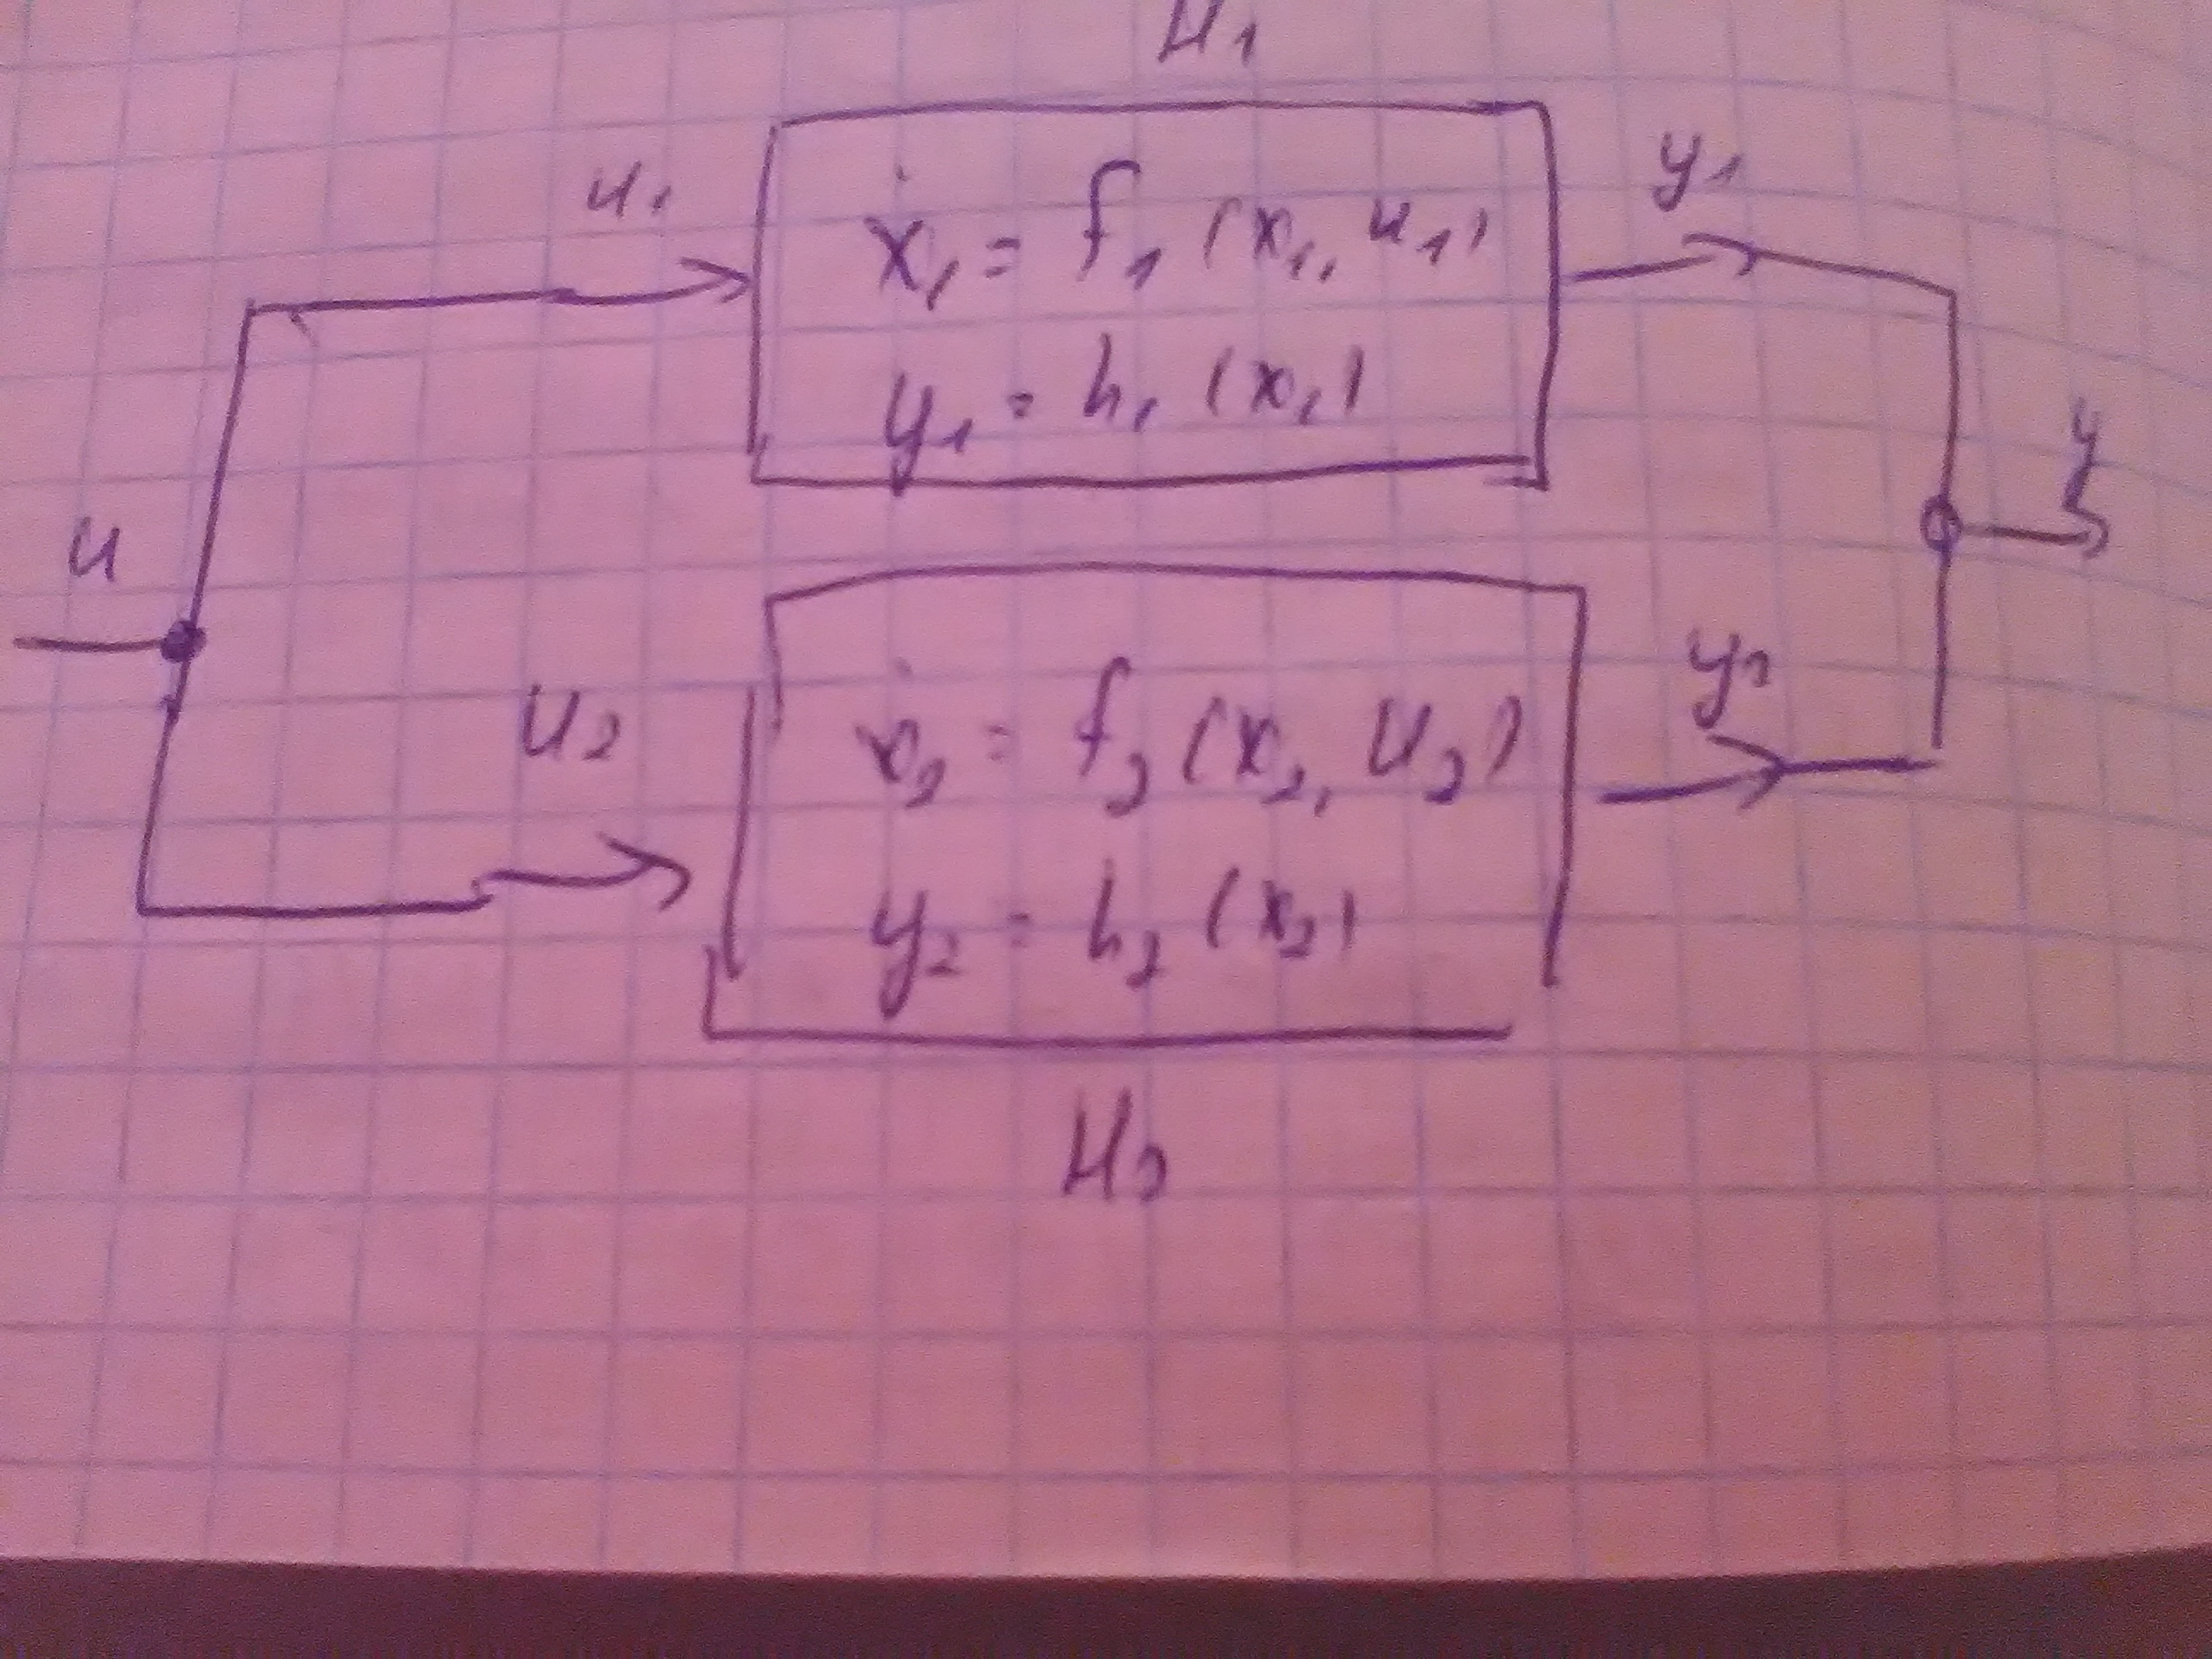
\includegraphics[scale=0.1]{3}
\end{center}

Take $S(x_1,x_2) = S_1(x_1) +S_2(x_2)$.
\begin{equation*}
\dot{S} \leq u_1^Ty_1 + u_2^Ty_2 = u^T(y_1+y_2) = u^Ty
\end{equation*}
\item Feedback interconnection of passive systems are passive

\begin{center}
	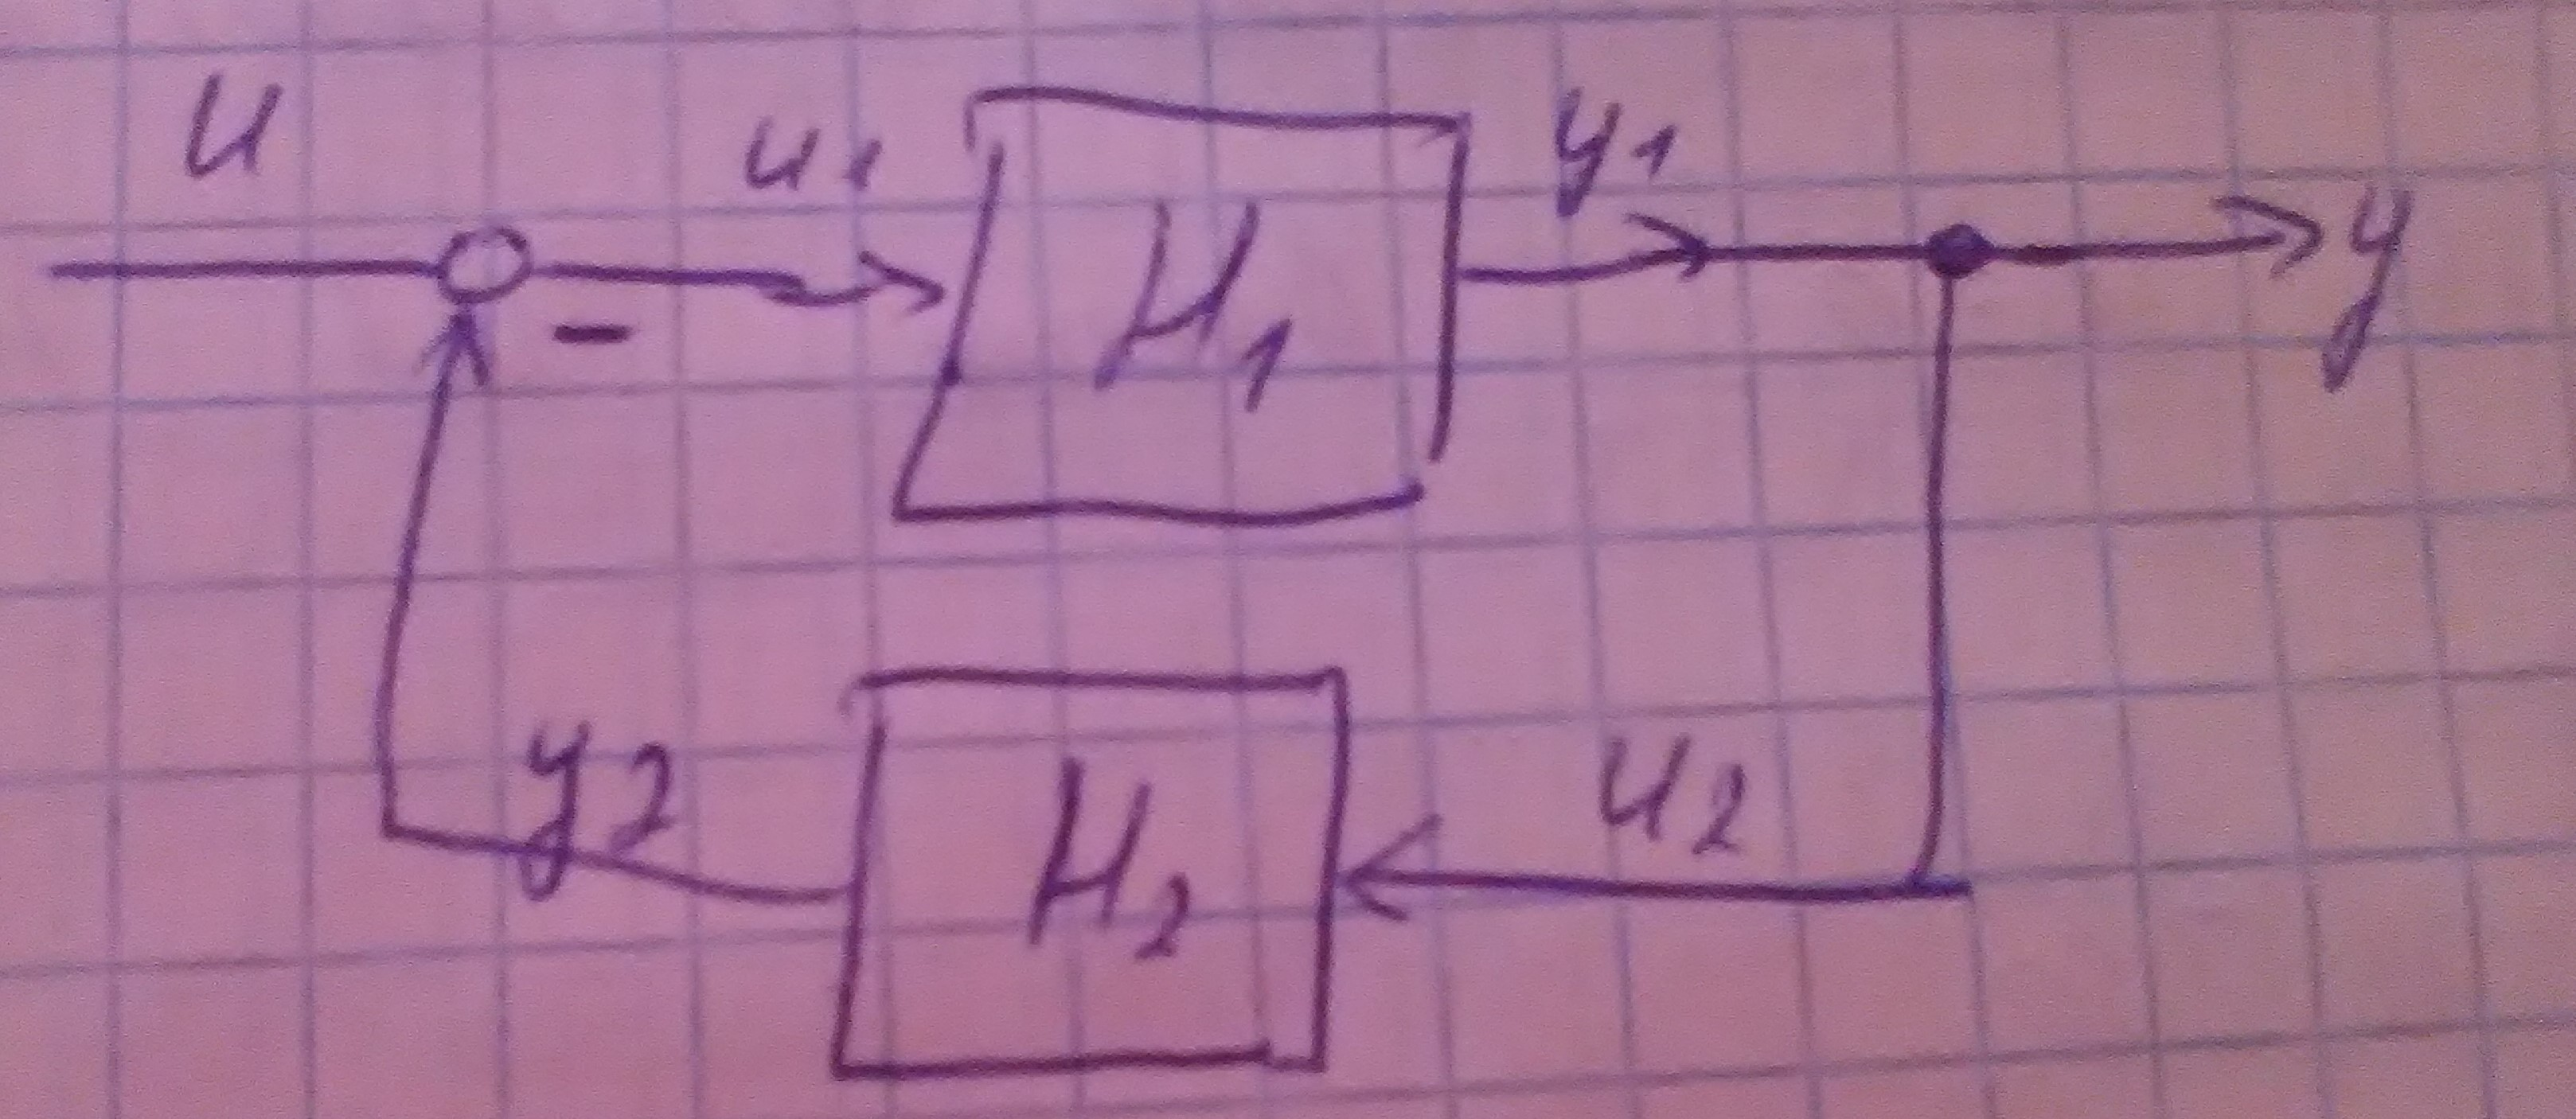
\includegraphics[scale=0.1]{4}
\end{center}

Take $S(x_1+x_2) = S_1(x_1) + S_2(x_2)$
\begin{equation*}
S \leq u_1^Ty_1 + u_2^Ty_2 =^{x_1=u_2=y} y^T(u_1+y_2) = y^Tu
\end{equation*}
\end{enumerate}

Remark:
\begin{itemize}
\item does not work for serious interconnections
\item can construct possibly large networks of passive systems
\end{itemize}

Stability if feedback interconnections:

Main idea: "shortage" of passivity of $H_1$ can be compensated by "excess" of passivity of $H_2$

\begin{Theorem}
Consider feedback interconnection (2) with $u \equiv 0$. Assume that $H_1$ and $H_2$ are (i) ZSO and dissipative with differentiable $S_1, \ S_2$ w.r.t. the supply rates
\begin{equation}\label{passivity_interconnection}
s_i(u_i,y_i) = u_i^Ty_i - \rho_iy_i^Ty_i - \nu_iu_i^Tu_i, \ i=1,2, \ \rho,\nu \in \mathbb{R}
\end{equation}
Then the origin $(x_1,x_2) = (0,0)$ for interconnection is asymptotically stable if $\nu_1 + \rho_2 > 0$ and $\nu_2 + \rho_1 > 0$.
\begin{proof}
Take $S(x) = S_1(x_1)+S_2(x_2)$.
\begin{equation*}
\begin{split}
\dot{S}(x) \leq^{(\ref{passivity_interconnection})} u_1^Ty_1 - \rho_1 y_1^Ty_1 - \nu_1u_1^Tu_1 \\
+ u_2^Ty_2 - \rho_2y_2^Ty_2 - \nu_2u_2^Tu_2 \\
= - (\rho_1 + \nu_2)y_1^Ty_1 - (\rho_2 +\nu_1)y_2^Ty_2
\end{split}
\end{equation*}

$u_1^Ty_1$ and $u_2^Ty_2$ can be excluded as $u_1=-y_2, \ u_2 = y_1$. 

$\Rightarrow$ can show as in previous theorem that $S$ is positive definite $\Rightarrow$ Lyapunov stability

For using La Salle:
\begin{equation*}
\begin{split}
y_1 \equiv 0 \Rightarrow u_2 \equiv 0 \Rightarrow^{ZSO} x_2 \equiv 0 \\
y_2 \equiv 0 \Rightarrow u_1 \equiv 0 \Rightarrow^{ZSO} x_1 \equiv 0
\end{split}
\end{equation*}
\end{proof}
\end{Theorem}

Remark
\begin{itemize}
 \item If (\ref{passivity_interconnection}) is sabisfied with $v_i=0$: "output - feedback passive" $\Rightarrow$ $p_i>0$
  -  "excess" of passivity, $p_i<0$ - "shortage" of passivity ($|p_i|$).
 \item If (\ref{passivity_interconnection}) satisfied with $p_i=0$: "input - feadforward passive" $\Rightarrow$ $v_i>0$
  -  "excess" of passivity, $v_i<0$ - "shortage" of passivity ($|v_i|$).
 \item Comment on terminology "output feedback passive" 
  $\dot s \le u^Ty-\rho y^Ty =$ [output feedback $u=\bar u -ky$] 
  $=\bar u^T y - (\rho+k)y^T y \le \bar u^Ty$ In other words, system can be made passive
  by output feedback.
 \item Similar for feedforward passivity, system can be made passive by feedback forward
  the input: $\bar y = y + ku$.
\end{itemize}

Remark:

Feedforward interconnection 2) can be extended to allow $h_1$ or $h_2$ to explicitly depend
on $u$ $\Rightarrow$ includes static systems (controllers) e.g. state output feedback $y=h(u)$
e.g. $y_2=ku_2$ $\Rightarrow$ input-strictly passive controller.

Extension of output-feedback/input-feedforward passivity:

$$s(u,y)=u^T-\rho(y)^Ty$$

with $\rho(y) = [\rho_1(y_1),\dots,\rho_n(y_n)]^T$ with $\rho_i$ section non-linearities, 
$\rho_i: \mathbb{R}\rightarrow\mathbb{R}$

\begin{Example}
\begin{equation*}
H_1: 
\begin{split}
 &\dot x_1 = x2 \\
 &\dot x_2 = -x_1^3 + x_2 + u \\
 &y = x_2
\end{split}
\end{equation*}

Take $S_1(x) = \frac{1}{4} x_1^4 + \frac{1}{2}x_2^2$ $\Rightarrow$ 
$\dot S_1 = x_1^3x_2 - x_1^3x_2 + x_2^2 + x_2u$, define $y^2:=x_2^2$ then
$yu=x_2u$ $\Rightarrow$ output - feedback passive with shortage of passivity 1
$\Rightarrow$ $\rho_1=-1$ and $v_1 = 0$.


\begin{tikzpicture}[auto,>=latex']
    \tikzstyle{block} = [draw, shape=rectangle, minimum height=3em, minimum width=3em, node distance=2cm, line width=1pt]
    \tikzstyle{sum} = [draw, shape=circle, node distance=1.5cm, line width=1pt, minimum width=1.25em]
    \tikzstyle{branch}=[fill,shape=circle,minimum size=4pt,inner sep=0pt]
    \tikzstyle{tmp} = [coordinate]
    %Creating Blocks and Connection Nodes
    \node at (-2.5,0) (input) {};
    \node [sum] (sum) {};
    %\node at (sum) (plus) {};
    \node [block, right of=sum] (u1) {$H_1$};
    \node [block, below of=u1] (k) {$k$};
    \node [tmp, right of=u1] (tmp1) {};
    \node [tmp, right of=k] (tmp2) {};
    \node [tmp, left of=k] (tmp3) {};
    %Conecting Blocks
    \begin{scope}[line width=1pt]
         \draw[->] (input) -- (sum);
         \draw[->] (sum) -- node{$u$} (u1);
         \draw[-] (u1) -- node{$y$} (tmp1);
         \draw[-] (tmp1) -- (tmp2);
         \draw[->] (tmp2) -- node{$u_2$} (k);
         \draw[-] (k) -- node{$y_2$} (tmp3);
         \draw[->] (tmp3) -| node[pos=0.99]{$-$} (sum);
    \end{scope}
\end{tikzpicture}

$y_2 = ku_2 \Rightarrow s(u_2,y_2)= \gamma ku_2^2 + \frac{1-\gamma}{k}y_2^2$,  $0<\gamma<1$ $\Rightarrow$ 
$\rho 2 = \frac{1-\gamma}{k}$, $v_2 = \gamma k$

$\Rightarrow v_2+\rho 1 > 0$ for $k>1$ and $\gamma$ close enough to 1, $v_1+\rho_2 = \rho_2 > 0$.
$\Rightarrow$ with ZSO, the origin is a stable.

\end{Example}